\documentclass[11pt]{article}

% Packages.
\usepackage[margin=1in]{geometry}
\usepackage{graphicx}
\usepackage{amsmath,amssymb,amsthm}
\usepackage{hyperref}
\usepackage{fancyhdr}
\usepackage{times}
\usepackage[final,nopatch=footnote]{microtype}
\usepackage{enumitem}
\usepackage{caption}
\usepackage{subcaption}
\usepackage{setspace}
\usepackage{listings}
\usepackage{xcolor}
\usepackage{algorithm}
\usepackage{algpseudocode}
\usepackage{booktabs}
\usepackage{multirow}
\usepackage{float}
\usepackage{ragged2e}
\usepackage{tikz}
\usepackage{titlesec}
\usetikzlibrary{positioning,arrows.meta,shapes}

% Metadata.
\hypersetup{
	pdftitle={CSI370: Verte Compiler - Assembly Refactor},
	pdfauthor={Andy Zheng},
	pdfsubject={Computer Architecture Software Project},
	colorlinks=true,
	linkcolor=blue,
	citecolor=blue,
	urlcolor=blue,
	pdfborder={0 0 0}
}

% Custom commands.
\newcommand{\coursecode}{CSI370}
\newcommand{\coursetitle}{Computer Architecture}
\newcommand{\assignmenttitle}{Software Project: Verte Compiler - Assembly Refactor}
\newcommand{\authorname}{Andy Zheng}
\newcommand{\authoremail}{andy.zheng@mymail.champlain.edu}
\newcommand{\institution}{Champlain College}

\newcommand{\code}[1]{\texttt{#1}}
\newcommand{\file}[1]{\texttt{#1}}
\newcommand{\constant}[1]{\texttt{#1}}

\newcommand{\verte}{\texttt{Verte}}
\newcommand{\vertec}{\texttt{vertec}}
\newcommand{\llvm}{\texttt{LLVM}}
\newcommand{\asm}{\texttt{x86-64 Assembly}}

\newcommand{\figref}[1]{Figure~\ref{#1}}
\newcommand{\tabref}[1]{Table~\ref{#1}}
\newcommand{\eqnref}[1]{Equation~\ref{#1}}
\newcommand{\lstref}[1]{Listing~\ref{#1}}
\renewcommand{\algref}[1]{Algorithm~\ref{#1}}

% Caption settings.
\DeclareCaptionType{eq}[][]

% Code listing style.
% stackoverflow.com/questions/741985/latex-source-code-listing-like-in-professional-books
\lstdefinestyle{codestyle}{
    basicstyle=\footnotesize\ttfamily,
    numberstyle=\tiny,
    numbersep=5pt,
    tabsize=2,
    extendedchars=true,
    breaklines=true,
    keywordstyle=\color{red},
    commentstyle=\color{blue},
    frame=top,
    stringstyle=\color{black}\ttfamily,
    showspaces=false,
    showtabs=false,
    xleftmargin=17pt,
    framexleftmargin=17pt,
    framexrightmargin=5pt,
    framexbottommargin=4pt,
    showstringspaces=false
}

\lstset{style=codestyle}

% Header/footer configuration.
\pagestyle{fancy}
\fancyhead{}
\fancyfoot{}
\fancyhead[L]{\small \coursecode\ --\ \assignmenttitle}
\fancyhead[R]{\small \authorname}
\fancyfoot[C]{\thepage}
\renewcommand{\headrulewidth}{0.4pt}

% Title page style.
\fancypagestyle{plain}{
	\fancyhf{}
	\fancyfoot[C]{\thepage}
	\renewcommand{\headrulewidth}{0pt}
}

% Custom styling.
\setlist[itemize]{label=$\diamond$, leftmargin=*}
\setlist[enumerate]{leftmargin=*}

% Adjust spacing.
\setlength{\parskip}{0.5em}
\setlength{\parindent}{0pt}
\setstretch{1.2}

% Enable numbering for paragraphs and subparagraphs.
\setcounter{secnumdepth}{5}
\setcounter{tocdepth}{5}

\titleformat{\paragraph}[hang]{\normalfont\normalsize\bfseries}{\theparagraph}{1em}{}
\titlespacing*{\paragraph}{0pt}{3.25ex plus 1ex minus .2ex}{1.5ex plus .2ex}

\titleformat{\subparagraph}[hang]{\normalfont\normalsize\bfseries}{\thesubparagraph}{1em}{}
\titlespacing*{\subparagraph}{0pt}{3.25ex plus 1ex minus .2ex}{1.5ex plus .2ex}

% Justify all text.
\justifying

\begin{document}
% Title page.
\title{\coursecode\ \coursetitle \\ \vspace{0.5em} \Large \assignmenttitle}

\author{
	\authorname \\
	\small \institution \\
	\small \texttt{\authoremail}
}

\date{\today}

\maketitle
\thispagestyle{plain}

\section{Project Overview}

\subsection{Project Description}

This project aims to refactor the existing code generation backend of the \vertec\ compiler. \vertec\ is a compiler built for the \verte\ programming language which beforehand utilized \llvm\ for machine code generation. With the implemented project, the \llvm\ backend was replaced with a custom \asm\ backend. This new backend directly translates the abstract syntax tree (\constant{AST}) created by the frontend layer into \asm\ instructions through several phases: \textbf{IR generation}, \textbf{register allocation}, \textbf{instruction selection}, and finally, \textbf{assembly generation \& compilation}.

\begin{figure}[h]
	\centering
	\small
	\setlength{\fboxsep}{6pt}
	\setlength{\fboxrule}{0.5pt}

	% Frontend.
	\textit{Verte Frontend}\\[0.4em]
	\fbox{\parbox{2cm}{\centering Source Code}}
	$\rightarrow$
	\fbox{\parbox{2cm}{\centering Lexer}}
	$\rightarrow$
	\fbox{\parbox{2cm}{\centering Parser}}
	$\rightarrow$
	\fbox{\parbox{2cm}{\centering AST}}
	\vspace{1.2em}

	% Current backend.
	\textit{Current Backend}\\[0.4em]
	\fbox{\parbox{2cm}{\centering LLVM IR Generator}}
	$\rightarrow$
	\fbox{\parbox{2cm}{\centering LLVM Optimization}}
	$\rightarrow$
	\fbox{\parbox{2.2cm}{\centering LLVM Backend}}
	\vspace{1.5em}

	% Implemented Backend.
	\textit{Implemented Backend}\\[0.4em]
	\fbox{\parbox{2cm}{\centering Custom IR Generator}}
	$\rightarrow$
	\fbox{\parbox{2cm}{\centering Register Allocation}}
	$\rightarrow$
	\fbox{\parbox{2cm}{\centering Instruction Selection}}
	$\rightarrow$
	\fbox{\parbox{2cm}{\centering Assembly Generator}}
	$\rightarrow$
	\fbox{\parbox{2cm}{\centering Compiler}}
	\vspace{1.2em}

	\caption{Verte Compiler Architecture with Proposed Backend}
	\label{fig:architecture}
\end{figure}

\subsection{Motivation}

The motivation behind this project comes from both educational and technical reasons. Firstly, I believe that building a custom assembly backend will provide a deeper understanding of low-level code generation, specifically a lot of theory can be read, but actually applying them is a different story; so I intend to see this as a checkpoint to verify my understanding of compiler design. Besides this, I also feel like it would be a good idea to explore alternatives to \llvm\ simply due to it's complexity and steep learning curve. Building a custom backend will alleviate this, and as a result of this, code generation will be more tailor-made, simplified, and understandable in contexts of maintaining the \verte\ programming language.

\subsection{Approach and Methodology}

The implementation of this refactor was carried out incrementally over several phases as mentioned in the project description. It first started with the analysis of the code base, and it's integration with the existing \llvm\ backend, this was done to best understand how to replace it without cascading changes through the existing code base for \verte. Following that, work was done incrementally based on the proposed backend outlined in \figref{fig:architecture}, starting with intermediate representation (\constant{IR}), to register allocation, instruction selection, and finally assembly generation and compilation. Whilst development was ongoing, unit tests were also added to cover critical components in the \asm\ compilation pipeline. This was done in order to ensure that development was technically correct, verifiable, and acceptable.

\section{Implementation}

\subsection{Intermediate Representation}

Like mentioned earlier, the first phase of the refactor involved designing and implementing a custom \constant{IR} to replace \llvm's \constant{IR} layer. This custom \constant{IR} follows the Three-Address Code (\constant{3AC}) format \cite{aho2007compilers} shown in \eqnref{eq:three-address-example}, over Static Single Assignment (\constant{SSA}) format, which is what \llvm\ uses. This choice was made because \constant{SSA} requires a $\phi$ function, the $\phi$ function can be thought of as a special merge operator in \constant{SSA} that handles control flow convergence. A general form of a $\phi$ function is show in \eqnref{eq:phi-example}.

\begin{eq}[!ht]
	\begin{equation}
		\label{eq:phi-example}
		\begin{aligned}
			x_3 = \phi(B_1: x_1, B_2: x_2)
		\end{aligned}
	\end{equation}
	\caption*{Equation 1: Phi-function Example}
\end{eq}

Where $B_1$ and $B_2$ are predecessor basic blocks, $x_1$ is the value of variable $x$ defined in block $B_1$, $x_2$ is the value of $x$ defined in block $B_2$, and $x_3$ is the merged result that takes the value of $x_1$ if control flow came from $B_1$, or $x_2$ if it came from $B_2$. While \constant{SSA} does enable certain optimizations for complex programs, it introduces additional complexity to maintain the single-assignment property. For the purposes of this refactor, the simpler \constant{3AC} format was deemed sufficient for \verte\ programs.

\newpage

The general form for \constant{3AC} can be represented as $x = y \texttt{ op } z$, where \texttt{op} represents the operator. At most, each instruction contains only three operands and no more. For example, \code{a = b + c * d} becomes:

\begin{eq}[!ht]
	\begin{equation}
		\label{eq:three-address-example}
		\begin{aligned}
			t_1 & = c \times d \\
			a   & = b + t_1
		\end{aligned}
	\end{equation}
	\caption*{Equation 2: Three-Address Code Example}
\end{eq}

In practice, the \vertec\ compiler generates $t_1$ as a virtual register. The \constant{IR} generator can assign an unlimited amount of virtual registers, which will then later be translated to physical registers through register allocation.

\subsubsection{Operand Types and Type Information}

In the \constant{IR} implementation, we have five distinct operand types: \textbf{virtual register}, \textbf{immediates}, \textbf{floating-point immediates}, \textbf{globals}, and finally \textbf{stack slots}. Each operand carries type information within it through the structure, \code{TypeInfo} rather than inferring types from context. This enables early error detection during the \constant{IR} generation phase, simplifies instruction selection by direct types, and facilitates automatic insertion of conversion instructions when mixing integer and floating-point arithmetic. Additionally to ensure the type-safe property of operands, the code base exposes factory methods shown in \lstref{lst:operand-creation} to construct these operands.

\begin{lstlisting}[language=C++, caption={Operand Creation with Type Information}, label={lst:operand-creation}]
		auto dest = ir::Operand::vreg(
    		vregID,
    		types::TypeInfo(types::TypeInfo::DataType::INTEGER)
		);
		

		auto foo = ir::Operand::imm(1);    // Implicit type.   
		auto bar = ir::Operand::fimm(1.0); // Implicit type.
		auto baz = ir::Operand::global(".str0");
		auto qux = ir::Operand::stackSlot(-8, intType);
	\end{lstlisting}

\subsubsection{Instruction Set}

In the \constant{IR} implementation we also define the instruction set able to be used by the compiler. The instruction set covers arithmetic for both integer and floating-point types (\constant{ADD}, \constant{SUB}, \constant{MUL}, \constant{DIV}, \constant{FADD}, \constant{FSUB}, ...), comparisons (\constant{ICMP\_LT}, \constant{FCMP\_EQ}, ...), type conversions (\constant{ITOF}, \constant{FTOI}), memory operations (\constant{LOAD}, \constant{STORE}), and control flow (\constant{BR}, \constant{CONDBR}, \constant{CALL}, \constant{RET}). These instructions are organized into basic blocks, of which only have a single entry and exit point. A basic block executes atomically, meaning if the first instruction runs, all instructions run in sequence. This property makes dataflow analysis much simpler as we can analyze the block as a unit.

\subsubsection{Control Flow Graphs}

Basic blocks are connected via predecessor and successor edges to form control flow graphs (\constant{CFG}). These control flow graphs are essential for the register allocation's liveness analysis. Consider the \verte\ conditional program shown in \lstref{lst:verte-example}.

\begin{lstlisting}[language=C, caption={Verte Conditional Example}, label={lst:verte-example}, numbers=none]
		fun main(): @int do
    		let x: @int = 1;
    		let y: @int = 2;
		
    		match where
        		when x == y do
            		return 0;
        		end
                
        		else -> return 1;
    		end
		end
	\end{lstlisting}

With this example \verte\ program, we can visually translate this into a \constant{CFG} shown in \figref{fig:cfg-example}, illustrating how control begins in block $B_1$, evaluates the condition, then takes one of two paths through $B_2$ or $B_3$, with both paths eventually converging at the exit.

\begin{figure}[H]
	\centering
	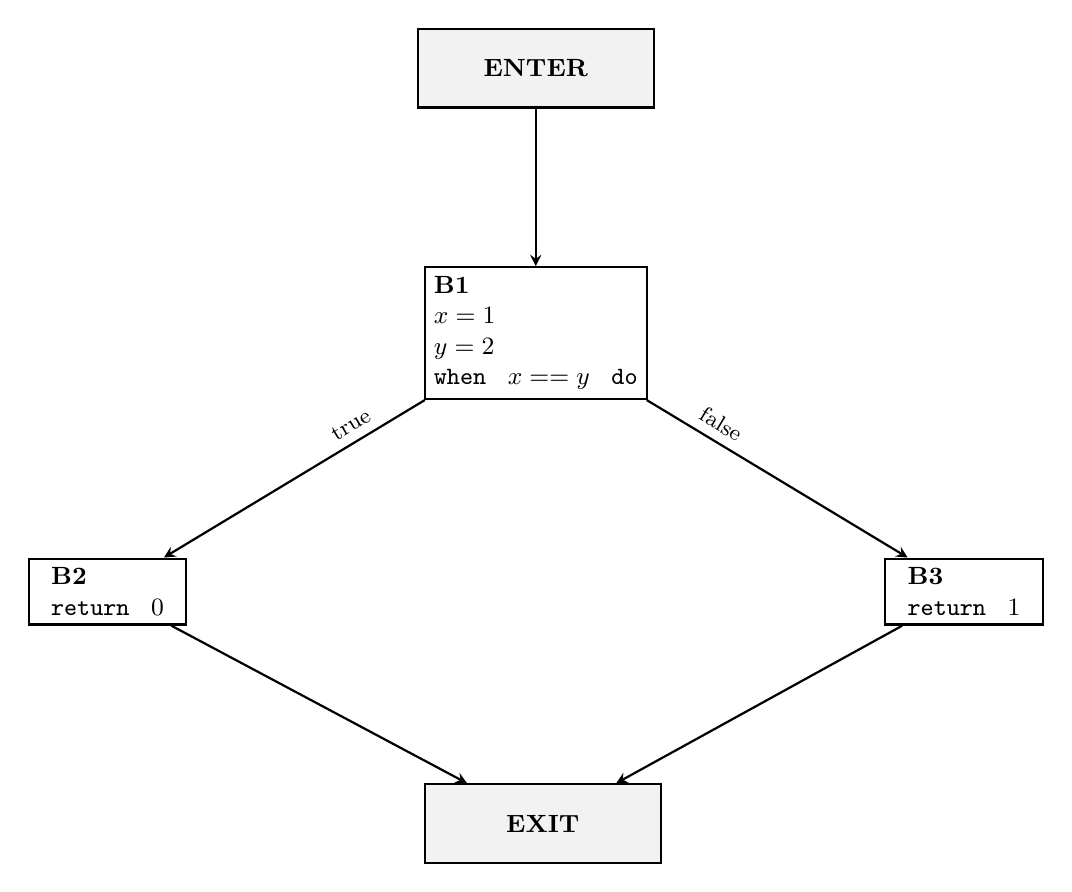
\begin{tikzpicture}[
			node distance=2cm and 3cm,
			block/.style={rectangle, draw, thick, minimum width=2cm, minimum height=0.5cm, align=left, font=\small},
			specialblock/.style={rectangle, draw, thick, minimum width=3cm, minimum height=1cm, align=center, font=\small\bfseries, fill=gray!10},
			arrow/.style={->, thick, >=stealth}
		]

		\node[specialblock] (enter) {ENTER};

		\node[block, below=of enter] (b1) {
			\textbf{B1}\\
			$x = 1$\\
			$y = 2$\\
			\texttt{when } $x == y$ \texttt{ do}
		};

		\node[block, below left=of b1] (b2) {
			\textbf{B2}\\
			\texttt{return } $0$
		};

		\node[block, below right=of b1] (b3) {
			\textbf{B3}\\
			\texttt{return } $1$
		};

		\node[specialblock, below right=of b2] (exit) {EXIT};

		\draw[arrow] (enter) -- (b1);
		\draw[arrow] (b1) -- node[left, near start, font=\footnotesize, sloped, above] {true} (b2);
		\draw[arrow] (b1) -- node[right, near start, font=\footnotesize, sloped, above] {false} (b3);
		\draw[arrow] (b2) -- (exit);
		\draw[arrow] (b3) -- (exit);
	\end{tikzpicture}
	\caption{Control Flow Graph for Conditional Statement}
	\label{fig:cfg-example}
\end{figure}

The algorithm to construct \constant{CFG}s in order to establish these predecessor and successor relationships is outlined in \algref{alg:cfg-construction}.

\begin{algorithm}[H]
	\begin{algorithmic}[1]
		\Procedure{BuildCFGLinks}{$func$}
		\For{each $block$ in $func.getBlocks()$}
		\State $terminator \gets$ last instruction in $block$
		\If{$terminator$ is branch}
		\State $target \gets$ branch target block
		\State link $block \rightarrow target$
		\ElsIf{$terminator$ is conditional branch}
		\State $trueTarget \gets$ true branch target
		\State $falseTarget \gets$ false branch target
		\State link $block \rightarrow trueTarget$
		\State link $block \rightarrow falseTarget$
		\EndIf
		\EndFor
		\EndProcedure
	\end{algorithmic}
	\caption{Control Flow Graph Construction}
	\label{alg:cfg-construction}
\end{algorithm}

\subsubsection{AST to IR Translation}

To actually construct the \constant{IR}, we use the \code{Codegen} class which implements the visitor pattern in order to traverse the \constant{AST}, generating \constant{IR} for each \constant{AST} node type. For example, binary operations translate as shown in \lstref{lst:binary-codegen}.

\begin{lstlisting}[language=C++, caption={Binary Operation IR Generation}, label={lst:binary-codegen}]
		auto Codegen::visit(const BinaryNode &node) -> RetT {
            auto lhs = std::get<ir::Operand>(node.getLHS()->accept(*this));
            auto rhs = std::get<ir::Operand>(node.getRHS()->accept(*this));
            const std::string &op = node.getOp();
			
            // Allocate result register.
            auto result = allocateVReg(lhs.getTypeInfo());
            
            ir::Opcode opcode;
			
            // Map operator to opcode.
            if (op == "+")
                opcode = ir::Opcode::ADD;
            else if (op == "-")
                opcode = ir::Opcode::SUB;
                
            // ... Additional operators ...
			
            currentBlock->addInstruction(
                ir::Instruction(opcode, result, lhs, rhs)
            );
            
            return result;
		}
	\end{lstlisting}

\newpage

\subsection{Register Allocation}

While the \constant{IR} generator is allowed to assign unlimited virtual registers, real CPUs only provide limited registers. To solve this we use a register allocation map to pair virtual registers with their physical counterparts. However, in the case that there are more live virtual registers compared to physical ones, some must be spilled to memory. To do this, we use an implementation of Linear Scan Allocation \cite{poletto1999linear}, which allocates registers in a single linear pass
over the program's live intervals.

\subsubsection{Live Interval Computation}

To use linear scan, we first need live intervals. A live interval spans from a virtual register's first definition to its last use as seen in \eqnref{eq:live-interval}. If two intervals overlap temporally, their registers will be unable to share the same physical registers. The algorithm computes intervals by numbering all instructions sequentially and tracking each virtual register's definition and last use indices.

\begin{eq}[!ht]
	\begin{equation}
		\label{eq:live-interval}
		\text{interval}(v) = [\text{firstDef}(v), \text{lastUse}(v)]
	\end{equation}
	\caption*{Equation 3: Live Interval Definition}
\end{eq}

In terms of implementation, \lstref{lst:liveness-compute} shows how this is done in practice.

\newpage

\begin{lstlisting}[language=C++, caption={Computing Live Intervals}, label={lst:liveness-compute}]
		std::vector<LiveInterval> 
		RegisterAllocator::computeLiveIntervals(const ir::Function &func) {
			std::unordered_map<uint32_t, size_t> firstDef, lastUse;
			std::unordered_map<uint32_t, bool> isFloat;
			
			// Number instructions and track usage.
			size_t position = 0;
			for (const auto &block : func.getBlocks()) {
				for (const auto &instr : block->getInstructions()) {
					// Track uses in operands.
					for (const auto &operand : instr.getOperands()) {
						if (operand.isVReg()) {
							lastUse[operand.getVRegID()] = position;
						}
					}
					
					// Track definitions in destination.
					if (instr.getDest().isVReg()) {
						uint32_t vreg = instr.getDest().getVRegID();
						if (!firstDef.count(vreg)) {
							firstDef[vreg] = position;
						}
                        
						lastUse[vreg] = position;
						isFloat[vreg] = isFloatType(
						  instr.getDest().getTypeInfo()
						);
					}
                    
					position++;
				}
			}
			
			// Construct intervals from tracking data.
			std::vector<LiveInterval> intervals;
			for (auto& [vreg, start] : firstDef) {
				intervals.emplace_back(
				    vreg, start, lastUse[vreg], isFloat[vreg]
				);
			}
			
			return intervals;
		}
	\end{lstlisting}

\subsubsection{Linear Scan Algorithm}

With the intervals computed and sorted by start position, the linear scan algorithm processes them in order. For each interval, it first expires any currently active intervals that have ended (freeing their registers), then it attempts to allocate a register from the appropriate free pool of registers (integer or floating-point). When no registers remain, the algorithm must spill to memory. \algref{alg:linear-scan} outlines the complete process.

\begin{algorithm}[h]
	\begin{algorithmic}[1]
		\Procedure{LinearScan}{$intervals$}
		\State Initialize $freeIntRegs \gets$ \{R10, ...\}
		\State Initialize $freeFloatRegs \gets$ \{XMM8, ...\}
		\State Initialize $active \gets \emptyset$
		\For{each interval $i$ in sorted intervals}
		\State \Call{ExpireOldIntervals}{$i$, $active$, $freeIntRegs$, $freeFloatRegs$}
		\If{$i.isInt$}
		\State $freeRegs \gets freeIntRegs$
		\Else
		\State $freeRegs \gets freeFloatRegs$
		\EndIf
		\If{$freeRegs \neq \emptyset$}
		\State $reg \gets$ pop from $freeRegs$
		\State assign $reg$ to $i$
		\State add $i$ to $active$
		\If{$reg$ is callee-saved}
		\State track $reg$ for prologue/epilogue
		\EndIf
		\Else
		\State \Call{SpillInterval}{$i$, $active$}
		\EndIf
		\EndFor
		\EndProcedure
	\end{algorithmic}
	\caption{Linear Scan Register Allocation}
	\label{alg:linear-scan}
\end{algorithm}

When all registers are exhausted, spilling becomes necessary. Spilled registers receive stack slots at negative offsets from the frame pointer: the first spill gets \code{[rbp - 8]}, the second \code{[rbp - 16]}, and so on. The decision of which interval to spill is made by checking if the current interval ends before all active intervals (since it has the shortest remaining lifetime); otherwise, spill the active interval with the furthest endpoint (which would occupy a register for the longest time).

\newpage

\subsection{Instruction Selector}

After \constant{IR} generation and register allocation on that \constant{IR}, in order to have a proper \asm\ program we must select \asm\ instructions to represent our \constant{IR} in code. We do this through pattern matching, essentially each \constant{IR} opcode maps to an assembly string. This assembly string is produced through dedicated selection functions for each type of \constant{IR} instruction.

\subsubsection{Two-Address Form Translation}

\asm\ arithmetic instructions uses the Two-Address form, where one operand serves two roles, being both source and destination. The \constant{3AC} \constant{IR} instructions $r_3 = r_1 + r_2$ cannot be directly translated to \code{add r3, r1}. The correct sequence requires an explicit copy shown in \lstref{lst:two-address}.

\begin{lstlisting}[language={[x86masm]Assembler}, caption={Two-Address Form Conversion}, label={lst:two-address}, numbers=none]
		mov r3, r1
		add r3, r2
	\end{lstlisting}

We apply this pattern to all binary operations to ensure we correctly translate our \constant{3AC} \constant{IR} code to \asm\ code.

\subsubsection{Function Calls}

Function calls are done through compliance with the System V ABI. The calling convention denotes exact register usage, and implementation wise we must strictly follow it. A critical requirement is the stack pointer alignment. The \constant{ABI} requires that \code{RSP} must be aligned to a 16-byte boundary before the \constant{CALL} instruction is executed. Since \constant{CALL} pushes an 8-byte return address, and our function prologue pushes \code{RBP} (8 bytes), we must be careful with calculation and tracking. The implementation in \lstref{lst:call-impl} demonstrates how this was done.

\begin{lstlisting}[language=C++, caption={Function Call Code Generation}, label={lst:call-impl}]
        void InstructionSelector::selectCall(
            const ir::Instruction &instr,
            const RegisterAllocator &allocator,
            std::vector<X86Instruction> &code
        ) {
            const auto &args = instr.getOperands();
            const std::string &funcName = instr.getFuncName();
            
            size_t intArgIndex = 0;
            size_t floatArgIndex = 0;
            size_t stackArgs = 0;
            
            // Calculate stack space needed for stack arguments.
            for (size_t i = 0; i < args.size(); ++i) {
                bool isFloat = isFloatType(args[i].getTypeInfo());
                if ((isFloat && floatArgIndex >= 8) || 
                (!isFloat && intArgIndex >= 6)) {
                    stackArgs++;
                }
                
                isFloat ? floatArgIndex++ : intArgIndex++;
            }
            
            // Align stack to 16 bytes if needed.
            size_t stackSpace = stackArgs * 8;
            if (stackSpace % 16 != 0) {
                stackSpace += 8;
            }
            
            if (stackSpace > 0) {
                code.push_back(X86Instruction("sub", "rsp", std::to_string(stackSpace)));
            }
            
            // Reset indices for actual argument passing.
            intArgIndex = 0;
            floatArgIndex = 0;
            size_t stackOffset = 0;
                        
            // Pass arguments.
            for (const auto &arg : args) {
                std::string argStr = formatOperand(arg, allocator);
                bool isFloat = isFloatType(arg.getTypeInfo());
                
                if (isFloat && floatArgIndex < 8) {
                    std::string xmmReg = 
                        getRegName64(FLOAT_ARG_REGS[floatArgIndex++]);
                    code.push_back(X86Instruction("movsd", xmmReg, argStr));
                }
                
                else if (!isFloat && intArgIndex < 6) {
                    std::string intReg = 
                        getRegName64(INT_ARG_REGS[intArgIndex++]);
                    code.push_back(X86Instruction("mov", intReg, argStr));
                } 
                
                else {

                    std::string stackLoc = 
                        "[rsp + " + std::to_string(stackOffset) + "]";
                        
                    std::string instr = isFloat ? "movsd" : "mov";
                    code.push_back(X86Instruction(instr, stackLoc, argStr));
                    stackOffset += 8;
                }
            }
            
            // Call the function.
            code.push_back(X86Instruction("call", funcName));
            
            // Clean up stack space.
            if (stackSpace > 0) {
                code.push_back(
                    X86Instruction("add", "rsp", std::to_string(stackSpace))
                );
            }
            
            // Move return value to destination register.
            if (instr.getDest().isVReg()) {
                std::string destStr = formatOperand(instr.getDest(), allocator);
                bool isFloat = isFloatType(instr.getDest().getTypeInfo());
                std::string retReg = isFloat ? "xmm0" : "rax";
                
                if (destStr != retReg) {
                    std::string instr = isFloat ? "movsd" : "mov";
                    code.push_back(X86Instruction(instr, destStr, retReg));
                }
            }
        }
    \end{lstlisting}

\subsection{Generation and Compilation}

So far, what has been described generally is the individual components of the compiler pipeline shown in \figref{fig:pipeline}. We are now at the final stage of that process, in this phase \constant{NASM} \asm\ files are created from the selected instructions through the assembly generator, then external tools are called to assemble and link the results into executable programs.

\begin{figure}[h]
	\centering
	\small
	\setlength{\fboxsep}{6pt}
	\setlength{\fboxrule}{0.5pt}

	\fbox{\parbox{2cm}{\centering IR Module}}
	$\xrightarrow{\text{Register Allocator}}$
	\fbox{\parbox{2.2cm}{\centering Allocated Functions}}
	$\xrightarrow{\text{Instruction Selector}}$
	\fbox{\parbox{2cm}{\centering Assembly Instructions}}

	\vspace{0.5em}

	\fbox{\parbox{2cm}{\centering Assembly Instructions}}
	$\xrightarrow{\text{Assembly Generator}}$
	\fbox{\parbox{1.5cm}{\centering .asm File}}
	$\xrightarrow{\text{NASM}}$
	\fbox{\parbox{1.3cm}{\centering .o File}}
	$\xrightarrow{\text{GCC}}$
	\fbox{\parbox{1.3cm}{\centering a.out File}}

	\caption{Compilation Pipeline Stages}
	\label{fig:pipeline}
\end{figure}

\subsubsection{Assembly File Generation}

The assembly generator starts by emitting the data section which contains initialized read-only data, such as floating-point constants and string literals. After this, the bss section is emitted and is reserved for uninitialized data, although currently unused in our implementation as globals are required to be constants in \verte. Then finally, the text section is emitted which contains the executable code for all functions.

Each function in the assembly code follows the standard structure. The prologue establishes the stack frame by pushing the base pointer, setting up \code{RBP}, allocating stack space, and saving callee-saved registers that were used by the register allocator. The function body contains the selected instructions translated to assembly code. The epilogue restores callee-saved registers, deallocates the stack frame, and returns control to the caller. A minimal example of this structure is shown in \lstref{lst:asm-structure}.

\begin{lstlisting}[language={[x86masm]Assembler}, caption={Assembly Function Structure}, label={lst:asm-structure}]
        section .text
            global main
        
        main:
            push rbp     ; Save old base pointer.
            mov rbp, rsp ; Set up new frame.
            sub rsp, 32  ; Allocate stack space.
        
            ; Function body.
        
            mov rsp, rbp ; Deallocate stack.
            pop rbp      ; Restore base pointer.
            ret
    \end{lstlisting}

\subsubsection{Compilation Pipeline}

After assembly generation, the compilation pipeline calls on external tools to produce an executable from the generated \asm\ file. It first determines the file paths for the assembly and object file, using the base name from the output path. The pipeline then executes sequentially the three stages shown in \figref{fig:pipeline}

The first stage calls the assembly generator's \code{writeToFile} method, which generates the complete \asm\ file and writes it to disk. This stage combines all previously computed information, that being the allocated registers, selected instructions, and constants table into a single assembly file. If this stage fails, the pipeline terminates immediately with an error.

The second stage calls \constant{NASM} through the \code{runAssembler} method. The command executed is \code{nasm -f elf64 -o output.o output.asm}, which assembles the generated assembly file into an \constant{ELF64} object file. If assembly fails, intermediate files are cleaned up based on compiler options passed by flags to \vertec.

The final stage calls \constant{GCC} through the \code{runLinker} method with the command \code{gcc -o output output.o -no-pie -z noexecstack}. The \code{-no-pie} flag disables position-independent executable generation, simplifying address calculations in our generated code. The \code{-z noexecstack} flag marks the stack as non-executable, a security feature that prevents code execution from stack memory. If linking succeeds and the compiler options do not request preservation of intermediate files, the pipeline automatically removes the temporary assembly and object files, leaving only the final executable.

\section{Challenges}

\subsection{Parameter Register Allocation Strategy}

Function parameter handling was not so trivial. In the System V ABI calling convention, parameters arrive in designated argument registers: \code{RDI}, \code{RSI}, \code{RDX}, \code{RCX}, \code{R8}, and \code{R9} for integers, and \code{XMM0} through \code{XMM7} for floating-point values. However, several of these registers are caller-saved, meaning they can be freely overwritten by called functions without preservation. This creates a problem when a parameter's value must survive across function calls within the body.

The initial register allocation implementation treated parameter virtual registers like any other virtual register, often assigning them to caller-saved registers like \code{R10} or \code{R11}. When the function subsequently called another function, these parameter values would be clobbered, producing incorrect results. The issue manifested subtly in recursive functions or functions with multiple internal calls that needed to reference parameters after making those calls.

The solution involved biasing the register allocator to prefer callee-saved registers (\code{RBX}, \code{R12}, \code{R13}, \code{R14}, \code{R15}) for function parameters. These registers are preserved across function calls by convention, as any called function must save and restore them. By allocating parameters to callee-saved registers, their values naturally survive function calls without requiring explicit saves and restores. The trade off is that using callee-saved registers requires the prologue to save them and the epilogue to restore them, adding overhead. However, this cost is typically cheaper than repeatedly spilling and reloading parameter values around each function call.

\newpage

\section{Conclusion}

This project successfully replaced \llvm\ with a custom \asm\ backend for the \vertec\ compiler. The implementation demonstrates fundamental compilation techniques: \constant{3AC} \constant{IR} design, linear scan register allocation, pattern-based instruction selection, and \constant{ABI} compliant assembly generation. It is fair to say that the educational value of this project has far exceeded initial expectations.

For example, designing the \constant{IR} showed how intermediate representations must balance abstraction with practical code generation concerns. Not to mention each decision about operand types, instruction formats, and control flow structures influenced every subsequent phase, demonstrating how foundational choices cascade throughout a compiler. On the other hand implementing register allocation brought forth the constraints of physical hardware into view. The naive and simple abstraction of unlimited virtual registers collides harshly with the reality that is finite physical registers, forcing decisions to be made on which values to keep in registers, and which to spill into memory. Beside this, instruction selection exposed just how wide the gap between high-level operations and actual machine code can be. Operations that seem simple in \constant{IR} notation often translate to multiple \asm\ instructions that need to be carefully orchestrated, each with its own register requirements and side effects. This aspect was seen a lot while working with the \constant{ABI}, and it definitely reinforced the idea that conventions exist for good reasons. Even small deviations from the expected calling conventions lead to subtle bugs that manifest only in specific circumstances, making them frustrating to diagnose.

The new backend, while certainly less optimized than \llvm, offers valuable experience and transparency in return. Every transformation is visible and understandable, making it possible to trace exactly how source code becomes machine code. This clarity proved invaluable during development and will continue to benefit future maintenance and enhancement. The code base now provides a solid foundation for further exploration, whether that involves adding optimization passes, experimenting with different register allocation strategies like graph coloring, or extending support to additional target architectures beyond \asm.

\newpage

% Bibliography.
\begin{thebibliography}{9}
	\bibitem{aho2007compilers}
	Aho, A. V. (2007). 6.2 Three-Address Code. In \textit{Compilers: Principles, Techniques \& Tools}.

	\bibitem{poletto1999linear}
	Poletto, M., \& Sarkar, V. (1999). Linear Scan Register Allocation. \textit{ACM Transactions on Programming Languages and Systems Volume 21, Issue 5}.
\end{thebibliography}
\end{document}
